\chapter{Communities with network motifs}
\label{ch:motifs}

The last chapter asked how finely a network can be divided, and answered it with
two priors over the same object. This one asks a different question: what the
divider is allowed to \emph{know} about the thing it is dividing.

Start with cycles, because they are where a network's local structure shows
itself. Every network has cycles of every length, and their numbers are not
remotely comparable: the yeast interactome holds a couple of hundred triangles
and ten thousand cycles of length eight, and a duplication--divergence network of
two hundred nodes holds none of length three, five or seven and seven million of
length eight. The counts climb steeply with length, and the steepness is not a
free parameter --- it is set by the short cycles.

That is the fact this chapter is built on, and it is worth stating at the outset.
The number of $h$-cycles through a node of degree $k$ is fixed by the degree
distribution together with one three-point quantity, the clustering coefficient,
and the length enters only as an exponent: the same closing probability applied
$h-2$ times around the loop (Section~\ref{sec:gr-conjecture}). Long cycles are not an
independent feature of a network. They are what short cycles compound into. A
description that has the triangles right has the whole spectrum right, wherever
triangles exist at all.

Wherever they do not, the compounding starts from something else, and the
question of \emph{which} something else turns out to be answerable by
measurement. A rule that closes squares rather than triangles leaves a spectrum
with a different shape, and one that closes pentagons a different shape again.

All of which bears on communities in a way that is not obvious until it is
stated. A block model divides a network on the evidence of where its links fall.
Clustering is evidence: a knot of mutually connected nodes looks like a
community. But if the network was grown by a rule that closes triangles
everywhere, the knots are not communities at all, and a method that could
\emph{name} a triangle would have an innocent explanation available where a
method without one has only the partition. So the question of this chapter is
whether giving a community model a vocabulary of motifs changes what it reports.
The answer, worked out over the sections that follow, is that it usually changes
when communities appear and not how many there are --- but that on two rules out
of eight it does something larger, and moves the network into a different limit
class altogether.

The concern is not new, and neither is the vocabulary. Recurring small subgraphs
were named \emph{network motifs} by \citet{milo2002}, who found them at
frequencies no random graph with the same degrees would produce; random graph
ensembles built to contain prescribed subgraphs rather than prescribed links were
constructed by \citet{karrer2010subgraphs}, and the model of
Section~\ref{sec:gr-motifsbm} is a block-structured version of theirs. Closest of
all, \citet{peixoto2022triadic} put exactly the suspicion above to work: a block
model in which each link is generated either by community membership or by
triadic closure over an existing path, with the assignment inferred alongside the
partition. On real networks it removes a good deal of what a plain block model
had been calling community structure. What follows differs in two ways. The
alphabet is not fixed to the triangle --- squares and bicliques are in it too,
because Chapter~\ref{ch:duplication}'s rules do not close triangles --- and the
target is not any one network but the \emph{scaling}, how the number of
communities grows with size and whether that exponent is a property of the
network or of the vocabulary used to describe it.

\section{Why a few motifs might be enough}
\label{sec:gr-conjecture}

Chapter~\ref{ch:graphons} ended by conjecturing that a locally grown network
converges to no kernel on the unit square at all, of two arguments or of any
number, and that what characterises its limit is instead intensive: a density of
communities, constant in size and set by the rule. It reached that conclusion by
abandoning an earlier guess --- that the limit is a kernel of \emph{higher
arity}, three arguments where the rule closes triangles and four where it
duplicates, with the fitted block model as the two-variable shadow of it.

This section takes the abandoned guess seriously for as long as it is useful,
which is not all the way. Its purpose is not to settle what the limit object is;
that question is left where Chapter~\ref{ch:graphons} left it. Its purpose is to
license an instrument. If a two-variable description can be shown to lose
something with a definite shape, and the shape can be shown to be fixed by the
shortest cycle the rule closes, then the way to build a better community model is
not to raise the arity of everything --- which is unaffordable, as we shall see
--- but to hand the ordinary pair model a small vocabulary of short motifs. That
is the conjecture this section exists to state. Everything after it is a test of
the instrument, not of the conjecture.

\subsection*{What a two-variable fit loses}

Take the two lattices whose construction is known exactly, so that every quantity
can be computed rather than estimated.

\begin{calculation}{the higher-order structure a two-variable model can hold}
The pseudofractal web of \citet{dorogovtsevgoltsev2002} has $n=(3^{t+1}+3)/2$
nodes and $3^{t+1}$ links, and every node added closes exactly one triangle, so
it holds exactly $n-2$ of them. Fit Chapter~\ref{ch:communities}'s branch cut and
ask each fitted model how many it expects, via $\mathrm{tr}(P^3)/6$ for its
expected adjacency matrix $P$.

The plain block model assigns one density per block pair. In a sparse network
those densities fall like $1/n$, and a triple of blocks contributes
$n^3\times n^{-3}$: the expected count is $O(1)$, and numerically it
\emph{saturates} at $21.3$ triangles however large the web grows.

The degree-corrected model does better, and still fails. Its expected count
weights each block by the degree sum $Q_r=\sum_{i\in r}k_i(k_i-1)$ rather than by
its size --- $k(k-1)$ and not $k^2$, because a triangle leaves a node by a
different link than it entered by, and the fit holds the degrees fixed --- and
for this web $Q\sim4^{t}$ while the degree sum is $S\sim3^{t}$, so the count
grows as $(Q/S)^3\sim(64/27)^t$ against a truth growing as $3^t$. The deficit
diverges, as $(81/64)^{t}=n^{0.214}$. Allowing the number of blocks to grow as
the data demand, $B\propto n^{\beta}$, helps but does not close it: $B$ blocks of
$n/B$ nodes contribute $O(1)$ triangles each, hence $n^{\beta}$ in all, still
short of $\Theta(n)$ by $n^{1-\beta}$.

The diamond lattice moves the arity by one and makes the failure worse. It is
bipartite and holds no triangle at all; its rule replaces each link with two
parallel paths, so its motif is the four-cycle, and after $t$ generations it has
$m=4^t$ links, $n=(2\cdot4^t+4)/3$ nodes and exactly $4^{t-1}$ four-cycles ---
only those closed at the \emph{last} generation are still four-cycles, earlier
ones having had their links subdivided into longer loops. Evaluating
$\mathrm{tr}(P^4)/8$ on the same cut, the plain model again saturates, at
$81/4=20.25$ four-cycles for a lattice of any size. The degree-corrected model is
where the two lattices part company: its count is governed by the ratio of the
excess-degree sum to the degree sum, and for this lattice that ratio is not a
power of $n$ at all but
\begin{equation}
  Q/S \;=\; \sum_i k_i(k_i-1) \Big/ \sum_i k_i \;=\; t
  \label{eq:gr-QS}
\end{equation}
exactly, so the expected four-cycle count converges to $t^4/4$:
\emph{poly\-log\-arithmic} in $n$, against a truth growing as $n/6$. At $t=26$ the
lattice holds $1.1\times10^{15}$ four-cycles and the fitted degree-corrected
model expects $1.2\times10^{5}$ of them.
\end{calculation}

So a two-variable description preserves what the \emph{cut metric} sees --- the
yardstick the limit theory uses, which judges two networks close when no way of
splitting the nodes into two sets reveals a difference in the density of links
across the split, and so registers block densities, degrees, the evidence for a
partition, everything Chapter~\ref{ch:graphons} computed --- and loses the
higher-order structure entirely, by a margin that widens without bound.

The gap between the two lattices --- $n^{0.214}$ against $n/(\ln n)^4$ --- is the
one thing they genuinely differ in, and it is worth naming because it recurs. The
pseudofractal's degrees are wild, $\gamma\simeq2.585$, and a rank-one model with
hubs that extreme manufactures a great many triangles by accident: three links
that all happen to touch the same few enormous nodes close a triangle whether or
not any rule intended it. The diamond's degrees are milder, $\gamma=3$ exactly,
which is the marginal case where $\sum k_i^2$ outgrows $\sum k_i$ only
logarithmically --- and a rank-one model then has nothing to fake with. The
two-variable model's apparent grasp of higher-order structure is not a grasp at
all; it is borrowed from degree heterogeneity, and it fails as the degrees become
tame. That is the mechanism behind something already measured in
Section~\ref{sec:gr-clustering}, where the degree-preserving null came within a
factor of $1.9$ of the Internet's clustering, whose degrees are extreme, and fell
$356$ times short for co-authorship, whose degrees are not. Degree-corrected
models do not capture clustering. They capture it exactly where the degrees are
heavy enough to counterfeit it.

One warning for anyone testing this at accessible sizes: the failure is not
visible early, and it changes sign. At $n\simeq3000$ the degree-corrected model
\emph{over}counts triangles fivefold, and only past $n\sim10^8$ does it cross
over to undercounting. A study stopping at ten thousand nodes would conclude the
opposite of the truth.

\subsection*{What is lost has a shape}

Triangles and four-cycles are two points. Asking the question at every cycle
length turns the finding from a shortfall into something with more content ---
and it is the content that motivates the alphabet.

\begin{calculation}{why a two-variable model has a one-parameter spectrum}
For a model with independent links and expected adjacency $P$, the expected number
of $L$-cycles is $\mathrm{tr}(P^L)/2L$. When $P$ is a $K$-block fit this collapses
onto a $K\times K$ \emph{transfer matrix}
\begin{equation}
  T_{rs} \;=\; \omega_{rs}\sqrt{Q_rQ_s}
  \qquad\text{(degree-corrected)},
  \label{eq:gr-transfer}
\end{equation}
with $Q_r=\sum_{i\in r}k_i(k_i-1)$, and $T_{rs}=p_{rs}\sqrt{n_rn_s}$ for the plain
model, so that the count at every length is $\mathrm{tr}(T^L)/2L$. The entire motif
spectrum is generated by one small matrix, and for large $L$ it is
$\lambda^L/2L$ for the leading eigenvalue $\lambda$ --- a smooth geometric profile.
A two-variable model has no freedom to put a feature at one particular length,
whatever its blocks are doing.

The weight is $k(k-1)$ rather than $k^2$ because a cycle leaves a node by a
different link than the one it arrived on, and the degree-corrected fit holds the
degree sequence fixed: a node offers $k(k-1)$ ordered pairs of links, not $k^2$.
The one-block case is then $\langle k^2-k\rangle/\langle k\rangle$, which is the
leading eigenvalue of the \emph{non-backtracking} operator, which counts walks
forbidden to turn round and retrace the link they arrived on --- the natural
object for cycles, since a cycle never does. The distinction is invisible in the
limits taken above, where the ratio diverges and the $-1$ is lost, but it is
worth a factor of $25$ at $L=8$ on a real network, where the ratio is nearer $3$.
\end{calculation}

The lattices do nothing but put features at particular lengths. The diamond is
built from four-cycles and carries cycles of length $4$, $8$, $16$, and so on ---
and \emph{exactly none} at any other length. Counted directly at $t=5$: zero
$3$-cycles, $256$ four-cycles, zero at five, six and seven, $1024$ eight-cycles.
The fitted models, meanwhile, expect $8.3$ triangles, $42$ five-cycles and $104$
six-cycles under the plain fit, and $40$, $668$ and $2994$ under the
degree-corrected one, at lengths where the lattice contains nothing whatever.

So the failure is not that the numbers are too small. It is that a two-variable
model places mass at every length while a locally grown lattice places it at a
few, and no adjustment of blocks or degrees can move a smooth profile onto a
sparse set of lengths. What a richer description buys is not a bigger number but
the ability to have a shape --- and a \emph{shape} supported on a few short
lengths is exactly what a small alphabet of motifs is.

That the shape is generated by one eigenvalue also fixes how the two lattices
differ. For a degree distribution $p(k)\sim k^{-\gamma}$,
\begin{equation}
  \lambda \;\sim\; n^{(3-\gamma)/(\gamma-1)} \quad (\gamma<3), \qquad
  \lambda \sim \ln n \quad (\gamma=3),
  \label{eq:gr-lambda}
\end{equation}
which gives the pseudofractal's exponent $0.2619$ and the diamond's $Q/S=t$. One
quantity governs both earlier results: the deficit at length $L$ is of order
$n/\lambda^{L}$, undercounting while $\lambda^L<n$ and overcounting after. The
rank-one part does not describe higher-order structure at any length. It
manufactures a geometric series and happens to cross the truth once.

That crossing is a falsifiable prediction, and it was tested on $44$ real
networks, with cycles counted exactly at $L=3\ldots8$ and each fitted model
represented by a sample from it rather than by the formula. Half of it came back
confirmed, and it is the half the argument stands on: a fitted model's own motif
spectrum really is generated by its transfer matrix, the sampled counts sitting
on $\lambda^L/2L$ to within one per cent at every length
(Figure~\ref{fig:gr-crossover}a). Eq.~\eqref{eq:gr-transfer} is not an
approximation that degrades. The crossing itself does not survive: real networks
carry many more cycles than their rewirings at \emph{every} length alike --- five
times more at the median, four thousand times for a large co-purchase network ---
and the excess barely decays, the measured slope being about a tenth of
$-\ln\lambda$, with thirty-nine of forty-two networks departing from the
predicted slope by more than two standard errors
(Figure~\ref{fig:gr-crossover}b). The deficit is a level, not a slope. The
lattices' motif counts are extensive and flat in $L$, so dividing by a geometric
profile leaves a geometric deficit and a crossing; real networks' cycle counts
grow with $L$ at very nearly the rate their rewirings do. The crossing is a
property of the deterministic webs, and the $L^\ast$ formula should be read as a
statement about them.

\begin{figure}[t]
  \centering
  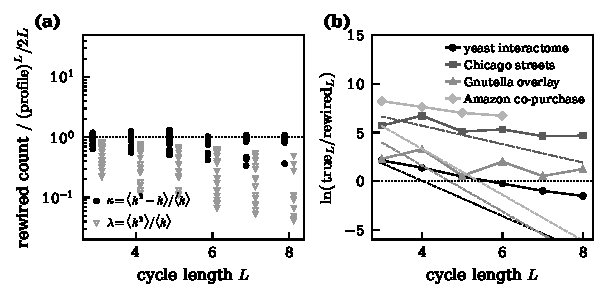
\includegraphics[width=\linewidth]{figs/fig-gr-crossover.pdf}
  \caption{The two halves of the prediction, on real networks. \textbf{(a)} A
  degree-preserving rewiring's own cycle counts, divided by the geometric profile
  its transfer matrix predicts. With the excess-degree branching factor
  $\langle k^2-k\rangle/\langle k\rangle$ the ratio sits on $1$ at every length;
  with $\langle k^2\rangle/\langle k\rangle$ it drifts away by an order of
  magnitude. \textbf{(b)} The deficit $\ln(\text{true}_L/\text{rewired}_L)$ for
  four systems, against the line of slope $-\ln\lambda$ through
  $L^\ast=\ln n/\ln\lambda$ that Eq.~\eqref{eq:gr-lambda} predicts (dashed). The
  measured curves are large and nearly flat.}
  \label{fig:gr-crossover}
\end{figure}

None of that touches the support argument, which the same measurement instead
strengthened by turning up a real network with the diamond's pathology.
Fullerenes are molecules, and their cycle spectra are exactly $12$ five-cycles
and $n/2-10$ six-cycles and \emph{nothing at any other length} --- twelve
pentagons at every size, which is Euler's theorem. Both fitted models put
positive mass everywhere: for $\mathrm{C}_{6000}$, five triangles, forty-three
four-cycles, twenty-seven seven-cycles. There the deficit is not fivefold or four
thousandfold, it is infinite in both directions, and no choice of blocks or
degrees can repair it.

\subsection*{How short a vocabulary has to be}

The shape is supported on a few lengths. How few, and which, is not something to
be postulated, because the cycle spectrum of a real network is already known to
be generated by a local quantity of arity three. Write $p_k$ for the degree
distribution and $c_k$ for the clustering coefficient of a node of degree $k$.
Then the number of $h$-cycles through a node of that degree
is~\citep{vazquez2005cycles}
\begin{equation}
  \frac{N_h}{n} \;=\; g_h\sum_{k}p_k\,\frac{(h-1)!}{2}\binom{k}{h-1}\,c_k^{\,h-2},
  \label{eq:gr-cycgen}
\end{equation}
with $g_h$ a correction for multiple counting: choose $h-1$ neighbours of a
central node, order them, and close the cycle by requiring $h-2$ links among
consecutive ones, each present with probability $c_k$. The degree distribution
and one three-point quantity fix the count at \emph{every} length, and the
measurement holds at $h=3,4,5$ across co-authorship, the Internet and a semantic
network~\citep{vazquez2005cycles}.

This is the licence the alphabet needs. The tower of longer cycles requires no
mechanism of its own: it is the product $c_k^{\,h-2}$, the same closing
probability applied $h-2$ times around the loop. Arity three buys not just the
triangle but the whole spectrum built from triangles, and for a great many real
networks triangles do the job.

They cannot do it for a network with no triangles. There $c_k=0$ identically,
Eq.~\eqref{eq:gr-cycgen} vanishes at every $h\ge3$, and the failure is not an
underestimate but an empty prediction --- against a network full of cycles. The
book's own duplication--split rule is exactly that case, built so that
duplication makes no triangles and splitting destroys any that might form.
Counting $DS(n,1/3)$ directly at $n=2000$: no triangles at all, then
$1.1\times10^4$ squares, $7.9\times10^3$ five-cycles and $1.3\times10^7$
eight-cycles. Nothing about the network is short of cycles; the arity-three
generator simply cannot see any of them.

So the order required is set by the shortest cycle the rule closes, and it is
measurable rather than postulated. The bubble family makes it a dial, since
$BB(n,L)$ closes a fresh cycle of length $L+2$ at every step:

\begin{center}
\begin{tabular}{llll}
\hline
model & motif & $c$ & cycle lengths present, $L=3\ldots10$\\
\hline
$BB(n,1)$ & triangle & $0.74$ & every length\\
$BB(n,2)$ & square & $0$ & $4,6,8,10$\\
$BB(n,3)$ & pentagon & $0$ & $5,8$\\
$BB(n,4)$ & hexagon & $0$ & $6,10$\\
\hline
\end{tabular}
\end{center}

\noindent Only the first is within reach of Eq.~\eqref{eq:gr-cycgen}. The others
place their mass exactly where the motif and its gluings put it: two faces
sharing a link close a cycle of length $a+b-2$, so pentagons give $5$ and $8$,
hexagons $6$ and $10$, and everything else is empty. That is the same arithmetic
the fullerenes obey --- twelve pentagons and $n/2-10$ hexagons at any size, then
$60$ nine-cycles and $3n/2-60$ ten-cycles, with seven and eight empty because no
two pentagons touch. A molecule and a growth rule, agreeing on a rule about which
templates may be adjacent.

\subsection*{The conjecture, and why not a tensor}

Three things have now been established, and together they say what to build. A
two-variable fit loses the higher-order structure by a diverging margin. What it
loses is not a number but a shape, supported on a few short lengths. And which
lengths are populated is fixed by the shortest cycle the rule closes, everything
longer following from it by compounding. Hence:

\begin{quote}
\emph{Conjecture.} A small alphabet --- the link, the triangle, the square, and
whatever else a rule's own footprint requires --- is sufficient vocabulary for
describing a locally grown network. Naming the shortest cycle a rule closes
accounts for the higher-order structure a two-variable model loses, and no
higher-arity object is needed to hold it.
\end{quote}

\noindent The alternative is to raise the arity of the model itself, and it is
worth saying why that is not done here. In the dense case the question is already
settled against it: an exchangeable array admits the representation
$f(\xi_\emptyset,\xi_i,\xi_j,\xi_{ij})$, and for a simple dense graph the
pair-level variable $\xi_{ij}$ can always be absorbed into a threshold, leaving a
two-variable kernel. Exchangeability \emph{forces} the graphon form; no
higher-order object can add anything. Whatever raising the arity buys, it cannot
be that, and its content lies entirely in the sparse regime --- which is the
regime this whole book is about, and the reason the clustering of
Section~\ref{sec:gr-clustering} does not vanish when a graphon says it must.
There the pair-level randomness does not wash out, and the natural object keeps
arguments indexed by \emph{pairs} rather than by nodes: not $W(x_i,x_j,x_k)$ but
something closer to $W(x_{ij},x_{ik},x_{jk})$, which is the shape the limit
theory of hypergraphs already takes. The inferential side of that idea has been
built: \citet{young2021hypergraph} ask, of an ordinary pairwise network, which of
its cliques are better explained as single higher-order interactions than as the
links they appear to be, and answer by description length. It is the same
accounting used below, with hyperlinks in place of motifs.

In practice, though, the tensor is unaffordable, and Chapter~\ref{ch:graphons}
priced it exactly: a block model over $j$-sets has a count tensor with about
$B^j/j!$ entries, and balancing that against what a split saves gives
$B_{\max}\approx[m(j-1)!/\ln m]^{1/j}$, which is $\sqrt n$ at $j=2$ and $n^{1/4}$
at $j=4$ --- eighteen groups where the pair model recovers three hundred and
sixteen (Eq.~\eqref{eq:gr-bmax}). A model that can no longer see communities is a
poor instrument for asking what communities are made of. The conjecture's virtue
is that it buys the shape without paying that price, and the next section builds
the instrument that follows from it.

\section{Fitting the order, not assuming it}
\label{sec:gr-motifsbm}

All of that still asks the reader to accept the arity of each rule as given. It
can instead be \emph{inferred}, by the same criterion that fits a block model in
the first place: minimum description length. The posterior of
Section~\ref{sec:gr-blockmodel} is \emph{microcanonical} --- it fixes the link
counts exactly rather than only on average, so that a model is a set of
constraints and the description length counts the networks satisfying them --- and
$\Sigma=-\log_2P(A,e,b)$ makes no use of the fact that links join two nodes. Nothing stops us handing it a
model built from something else.

\begin{calculation}{an alphabet of motifs, priced}
The obvious something else --- a block model over $4$-sets, its count matrix
replaced by a four-index tensor --- is the wrong choice, and
Section~\ref{sec:gr-twopriors} has already priced it: a $j$-index tensor drops the
resolution to $B_{\max}\approx[m(j-1)!/\ln m]^{1/j}$, which at $j=4$ is $n^{1/4}$,
eighteen groups where the pair model recovers three hundred and sixteen. A model
that can no longer see communities is a poor instrument for asking what
communities are made of.

The affordable object keeps the ordinary block structure and changes what the
blocks are built from. Every link is assigned to exactly one \emph{motif
instance} drawn from a small alphabet --- a link, a triangle, a square --- with
motifs of arity three and above planted inside a single block, and instances
wired by \emph{stub matching}: each node is given a number of loose link-ends,
or stubs, and the ends are then paired off at random, so that a node's share of
the motifs is fixed by how many stubs it was given. That generative recipe is
\citeauthor{karrer2010subgraphs}'s subgraph configuration model
\citeyearpar{karrer2010subgraphs}, run inside blocks. Planting $c$
copies of a motif that spans $s$ nodes inside one block can be done in
\begin{equation}
  \Omega \;=\; \frac{(sc)!}{\prod_i d_i!\;c!\;a^{c}}
  \label{eq:gr-omega}
\end{equation}
ways, where $d_i$ is how many of them node $i$ takes part in and $a$ is the size
of the motif's automorphism group --- the number of relabellings of its own nodes
that leave it unchanged, which is $2$ for a link, $6$ for a triangle and $8$ for
a square. Dividing by $a^{c}$ is what stops the same motif being counted once for
each way of writing it down. $\Sigma$ is then the sum of $\log_2\Omega$ over the
blocks together with the cost of the partition and of the counts. The parameters
number one count per motif type per block plus the block matrix, $3B+B^2$ for the
alphabet used here, rather than the $B^4/24$ of the tensor, so the
resolution ceiling stays at Eq.~\eqref{eq:gr-flatceiling}'s. The price is that a triangle straddling
two blocks is not representable and is described as three links instead.
\end{calculation}

Two features make this a test rather than a fitting exercise. With the alphabet
reduced to the link alone, $\Sigma$ is exactly the description length of the
ordinary degree-corrected model, so enlarging the alphabet is a strictly nested
comparison and a negative $\Delta\Sigma$ means the motifs paid for themselves. And
the criterion can tell a planted triangle from three incidental links, because
$c$ planted triangles are more constrained --- hence cheaper to specify --- than
the $3c$ independent links they account for, while the extra counts cost only a
little. Where triangles are unavoidable rather than planted the arithmetic goes
the other way, and on a nine-node graph carrying $26$ of its $36$ possible links
the criterion correctly plants none at all.

Run against the networks whose construction is known exactly, it recovers the
rule:

\begin{center}
\begin{tabular}{lrrl}
\hline
network & $n$ & $\Delta\Sigma$ (bits) & selected\\
\hline
pseudofractal, $t=5$      & 366 & $-398$ & triangle\\
$BB(n,1)$                 & 500 & $-259$ & triangle\\
diamond, $t=5$            & 684 & $-1032$ & square\\
$DS(n,1/3)$               & 500 & $-39$  & square\\
$BB(n,2)$                 & 500 & $-204$ & square\\
$BB(n,3)$, pentagons      & 500 & $+21$  & none\\
$BB(n,4)$, hexagons       & 502 & $+19$  & none\\
fullerene $\mathrm{C}_{240}$ & 240 & $+17$ & none\\
\hline
\end{tabular}
\end{center}

\noindent The last three rows are the ones that matter. Their motifs lie outside
the alphabet, and there the enlarged model costs bits and buys nothing --- the
$+17$ is precisely the price of announcing two totals that turn out to be zero.
It does not offer a square when the network was built from pentagons. A planted
network with triangles in one community and squares in another is recovered with
both, each in its own block; and the diamond at $t=4$ is decomposed into exactly
$64=4^{t-1}$ squares, the number it actually contains.

Two cautions. The decomposition assigns each link to one instance, so motifs that
overlap cannot all be represented: the pseudofractal holds $n-2$ triangles but at
most a third of its links' worth are disjoint, and $138$ were found. The
selection is meaningful; the counts are not estimates. And the search is greedy
in two coupled directions at once, which can trap it --- on the diamond, the
branch cut of Chapter~\ref{ch:communities} places \emph{every} four-cycle across
the cut, so from that partition the model finds no motif at all, and only a
different starting partition reveals them.

So the conjecture of Section~\ref{sec:gr-conjecture} holds up as far as the
instrument can be checked against networks whose construction is known. A symbol
of arity three pays for itself where the rule closes triangles, one of arity four
where it closes squares, and neither pays where the rule closes something longer
--- which is the conjecture's own statement, arrived at by measurement rather
than by assumption, and the alphabet is doing its job when it declines as well as
when it accepts. That is as much as the vocabulary question needs; what the
vocabulary then \emph{does} to a community count is a separate matter, and the
rest of the chapter is about that.

\section{Three limit classes}
\label{sec:gr-classes}

The instrument is built. It can be run on every rule in this book, and against
the two block models it contains as special cases, so that the same networks are
counted three ways: by a flat block model, by a nested one, and by the nested one
with an alphabet of motifs. What separates the three is worth pinning down before
the numbers arrive, because the whole chapter turns on it.

\begin{calculation}{the three methods, and what separates them}
All three minimize the same description length,
\begin{equation}
  \Sigma \;=\; -\log_2 P(A\,|\,\text{model}) \;-\; \log_2 P(\text{model}),
  \label{eq:gr-sigma}
\end{equation}
the bits needed to transmit the network together with the model used to compress
it, and all three infer the number of communities rather than being told it. All
three are also \emph{degree-corrected} in the sense of
Eq.~\eqref{eq:gr-factor}: each node carries its own propensity to link, so that a
hub and a leaf can sit in the same community without the fit having to separate
them on degree alone. Chapter~\ref{ch:communities} showed why that matters --- the
degree-blind fit cuts the pseudofractal into hubs and leaves rather than into
branches. With that held fixed, the three differ only in what the model is
permitted to say.

\emph{Flat block model.} Blocks, and a $B\times B$ matrix of link counts between
them under an uninformative prior. Describing that matrix costs about
$\tfrac12B^2\log_2 m$ bits for a network of $m$ links, which is what caps the
recoverable groups at $B_{\max}\propto\sqrt n$. This is the method of
Chapter~\ref{ch:communities}.

\emph{Nested block model.} The same, except that the matrix of link counts is
itself described by a block model, and that one by another, in a hierarchy. The
cost of the top-level description falls away and the ceiling rises to
$B_{\max}\propto n/\log n$ \citep{peixoto2014hier}.

\emph{Nested $+$ motifs.} The nested model, with every link additionally assigned
to one motif instance --- a link, a triangle or a square --- as in
Eq.~\eqref{eq:gr-omega}. With the alphabet reduced to the link alone this is
exactly the nested model, so the comparison is strictly nested and
$\Delta\Sigma<0$ means the motifs paid for themselves.

The first two differ in resolving power and nothing else; the second and third
differ in vocabulary and nothing else. So a change between the first two is about
how finely a method can see, and a change between the last two is about what it
is willing to call a community.
\end{calculation}

\noindent Two quantities are read off each fit. The first is
Chapter~\ref{ch:communities}'s Ramsey community number $r_\kappa$, the size at
which communities become certain --- $P_\kappa\ge0.95$ over a hundred
realisations up to $n=200$ and twenty above it --- which asks \emph{whether} a
network has communities. The second is Chapter~\ref{ch:graphons}'s exponent
$\beta$ in $\kappa\propto n^{\beta}$, which asks \emph{how many}. Here is
everything, for every rule, all three ways.

\begin{center}
\small\setlength{\tabcolsep}{4pt}
\begin{tabular}{llrrrrrrr}
\hline
 & & \multicolumn{3}{c}{$r_\kappa$, onset of communities} & \multicolumn{3}{c}{$\beta$, growth of $\kappa$} & links\\
rule & motif & flat & nested & $+$mot. & flat & nested & $+$mot. & named\\
\hline
\multicolumn{9}{l}{\emph{constant density}}\\
\quad $LS(n,1)$ & triangle & $70$ & $80$ & $200$ & $0.54$ & $0.94$ & $1.04$ & $62\%$\\
\quad $BB(n,1)$ & triangle & $90$ & $100$ & $400$ & $0.48$ & $0.89$ & $0.89$ & $54\%$\\
\quad $DS(n,1/3)$ & square & $300$ & $250$ & $250$ & $0.78$ & $0.92$ & $1.04$ & $26\%$\\
\quad $DS(n,0.5)$ & square & $90$ & $100$ & $100$ & $0.76$ & $1.02$ & $1.01$ & $12\%$\\
\quad $DD(n,0.5)$ & biclique & $40$ & $40$ & $40$ & $0.78$ & $1.12$ & $1.11$ & $0\%$\\
\quad pseudofractal & triangle & --- & --- & --- & $0.61$ & $1.02$ & $0.99$ & $56\%$\\
\hline
\multicolumn{9}{l}{\emph{no communities}}\\
\quad $BA(n,2)^{\dagger}$ & --- & never & --- & --- & --- & --- & --- & ---\\
\quad $BB(n,2)$ & square & $400$ & $400$ & never & $0.72$ & $0.97$ & --- & $57\%$\\
\hline
\multicolumn{9}{l}{\emph{fractal}}\\
\quad diamond & square & --- & --- & --- & $0.71$ & $1.05$ & $0.31$ & $92\%$\\
\hline
\end{tabular}
\end{center}


\noindent The motif column is the shortest cycle the rule closes --- $\triangle$
for a triangle, $\square$ for a square, $K_{2,d}$ for duplication's biclique,
which has no symbol and is the one motif in the book of no fixed size. The last
column is the fraction of a network's links that the alphabet actually succeeds
in naming at the largest size fitted, and it is there because it turns out to be
what decides the rest. The dagger marks the one row taken from
Chapter~\ref{ch:communities} rather than measured here.

The lattices need one remark, since they are deterministic --- one network per
generation, not a hundred realisations per size. For them $P_\kappa$ is a step
function rather than an estimate, so $r_\kappa$ is exactly the smallest
generation whose fit returns more than one group, and the only imprecision is the
grid: a lattice quadruples at every step, so the figures quoted are the first
generation past the onset and the true crossing lies somewhere in the factor of
four below. Their exponents are fitted from $n=366$ and $n=684$ upward, the
smaller generations being below the resolution of any of the three methods.

Read down the table and the rules fall into three classes, which are the
organising fact of this chapter and the three sections that follow.

\emph{No communities.} $P_\kappa$ never reaches certainty; the best description
uses a single group at arbitrarily large size. Chapter~\ref{ch:communities}'s
non-local control $BA(n,2)$ is the canonical member --- preferential attachment
with no step that ever looks at a neighbourhood, and no communities at any size.
It is the one row here not measured with this chapter's instrument, and is marked
accordingly: the ``never'' is that chapter's flat fit, and neither the nested
model nor the alphabet has been run on it, so it stands as the class's definition
rather than as a comparison. What is new is that a network with a perfectly good
local rule can be moved into the same class by nothing more than a change of
vocabulary. $BB(n,2)$ has a Ramsey number of $400$ under both block models and
none at all once its squares can be named, and both deterministic lattices go the
same way for a reason Section~\ref{sec:gr-square} makes exact.

\emph{Constant density.} $\beta=1$, so $b=\kappa/n$ stops depending on size and
becomes a number the rule has, in the sense of Chapter~\ref{ch:graphons}'s
Eq.~\eqref{eq:gr-density}. Five of the measured rules are here, the nested model
and the alphabet agreeing on every one of them to within about a tenth.

\emph{Fractal.} Communities emerge, their number grows, and the density does not
survive: $0<\beta<1$, so $b\to0$ as a power of the size. It is a coherent
possibility and no rule in this book occupies it. The diamond lattice appeared to
for a while, at $\beta=0.31$, and Section~\ref{sec:gr-square} is the account of
why it does not: the exponent was a partition the search was reporting and did
not need.

Three things about that classification need saying immediately, because they
qualify everything after it.

The first is that a class is a property of a network \emph{together with the code
used to describe it}, and the table shows this in the plainest possible way: two
of the eight rules change class when the vocabulary changes, and nothing about
the networks changes at all. This is the same lesson Chapter~\ref{ch:graphons}
learned twice --- once for the prior and once for the sample --- and it is
sharper here, because a prior moved an exponent while a vocabulary moves a rule
from one class to another.

The second is what the flat column says. Under the flat block model \emph{every}
rule in the table reads $\beta$ between $0.48$ and $0.78$: on that instrument the
whole book is in the fractal class. It is not. The flat model is sitting on its
own $\sqrt n$ ceiling, as Chapter~\ref{ch:graphons} established, and the apparent
fractality is the ceiling talking. Any claim that a network is in the third class
has to be made with a model that could have reported the first two --- and, as
the diamond turns out to show, with a fit one has some reason to think is the
best available.

The third is that the classification is a statement about the best description
anyone has found, and not about the best there is. That distinction is usually
academic and on the two lattices it is not: both were placed in other classes by
a fit that turned out to be beaten, at every size, by a decomposition one can
write down by hand. Section~\ref{sec:gr-square} does that, and the fractal class
is empty as a result. Where a better description is found, a row moves.

\section{The rules that keep their density}
\label{sec:gr-chapter6}

Five of the random rules are in the constant-density class, and they get there by
two quite different routes: either the alphabet names their motif and the density
survives anyway, or the alphabet cannot name it at all. Both routes are worth
following, because between them they say what the vocabulary is and is not able
to do.

Start with what naming a motif does to the \emph{onset}. The two rules
Chapter~\ref{ch:communities} published Ramsey numbers for are local search, at
$81$, and duplication--split, at $98$. The master table puts the first at $70$
under the flat model and $80$ under the nested one, and the second at $90$ and
$100$.

The two block-model columns bracket the published numbers without
quite reproducing them, and the gap is worth a word, since the flat column is
supposed to be Chapter~\ref{ch:communities}'s own method. It is the same method
in the sense that matters --- a degree-corrected block model, its number of groups
inferred by description length --- but that names a family of procedures rather
than one. The published figures come from a separate
implementation~\citep{vazquezcommunities2025}; the fit is a stochastic search
whose answer depends on how many restarts it is given and on the version of the
library doing it; $P_\kappa$ is estimated from a hundred realisations; and
$r_\kappa$ can only land on one of the sizes actually grown, here $\ldots70$,
$80$, $90$, $100\ldots$, so both published values fall one step above the flat
column. Agreement to a grid step is the check that this is the same measurement.
Equality was never on offer, and the columns to compare against each other are
the three measured here, which do share an implementation.

The motif alphabet then moves one of them and not the other. Local search
\emph{is} the triadic-closure rule, so its local structure is triangles; an
alphabet that contains the triangle books that structure as planted motifs
instead of reading it as evidence for communities, and the size at which
communities become certain is pushed from $80$ to $200$. Duplication--split makes
no triangles at all, its squares overlap heavily and compress little, and its
Ramsey number does not move (Figure~\ref{fig:gr-ramsey}).

\begin{figure}[t]
  \centering
  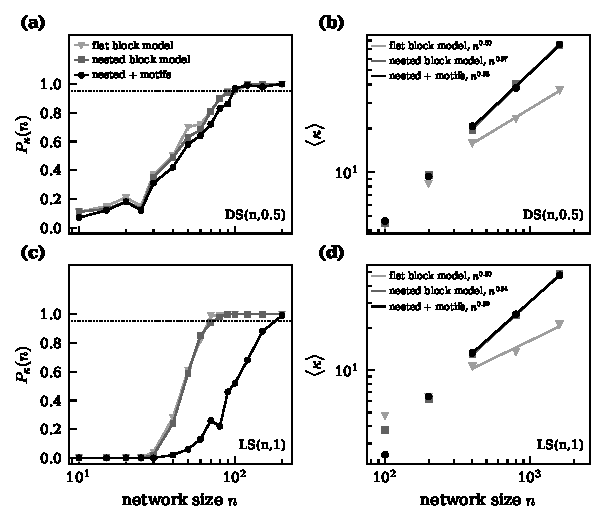
\includegraphics[width=\linewidth]{figs/fig-gr-ramsey.pdf}
  \caption{\textbf{The detection method is part of the answer.} Every panel
  compares three methods on identical networks: a flat block model, a nested one,
  and the nested one with triangles and squares in its alphabet.
  \textbf{(a)}~duplication--split, \textbf{(b)}~local search. The communities
  likelihood $P_\kappa(n)$, from a hundred networks at each size up to $n=200$
  and twenty above it, with the dotted line at the $95\%$ threshold whose
  crossing defines the Ramsey community number. Duplication--split makes no
  triangles and the three curves lie on top of one another; local search
  \emph{is} the triadic-closure rule, and naming its triangles moves the crossing
  from $80$ to $200$.}
  \label{fig:gr-ramsey}
\end{figure}

$BB(n,1)$, which closes triangles by a quite different mechanism --- laying a
single new node across a random link rather than closing a path --- behaves like
local search and not like its own square-closing sibling. Its onset moves from
$100$ to $400$ and nothing else happens: past the threshold the motif model's
community count converges on the nested model's rather than collapsing away from
it, $5.6$ against $5.8$ at $n=200$ and $11.1$ against $11.9$ at $n=400$, and its
exponent is $0.892$ with the alphabet against $0.886$ without it.

The pseudofractal web looks at first like the same story told deterministically
--- $1.02$ against $0.99$, a lattice built entirely of triangles whose density
appears untouched by being allowed to name them --- and it is not. That reading
comes apart in Section~\ref{sec:gr-square}, and it comes apart in a way that says
something about the instrument rather than about the lattice. It is left out of
this section for that reason, and so is the diamond.

So where the alphabet names the rule's own motif, it postpones the onset by a
factor of two to four and leaves the exponent alone. That is the first route into
this class, and the more informative one, because the alphabet was working and
the density survived anyway.

\subsection*{Where the alphabet names nothing}

The second route is duplication with divergence, and its entry in the table is
the $0\%$ in the last column: at $n=800$ the alphabet succeeds in naming
essentially none of the network's links. That is not for want of squares.
$DD(n,q)$ copies a random node and deletes each copied link independently with
probability $q$; it never subdivides anything, so unlike duplication--split it
stays bipartite, and counted directly at $q=\tfrac12$ it has mass at the even
lengths and exactly nothing at the odd ones:

\begin{center}
\begin{tabular}{lrrrrrr}
\hline
 & \multicolumn{6}{c}{number of cycles of length $L$}\\
$DD(n,\tfrac12)$ & $L=3$ & $4$ & $5$ & $6$ & $7$ & $8$ \\
\hline
$n=100$ & $0$ & $694$ & $0$ & $9\,099$ & $0$ & $123\,001$\\
$n=200$ & $0$ & $3\,658$ & $0$ & $143\,822$ & $0$ & $7\,002\,135$\\
\hline
\end{tabular}
\end{center}

\noindent By the reading of Section~\ref{sec:gr-conjecture} this is a square-built
network if ever there was one, and the motif model declines to plant a single
square in it. Fitted at $q$ from $0.2$ to $0.6$ the enlarged alphabet buys
nothing: it costs a few tens of bits on average, and the scatter between repeated
fits of the same network is larger than the cost, so the only thing the number
says is that nothing was gained.

The reason is that duplication does not make a square. It makes a node with $d$
shared neighbours --- a complete bipartite $K_{2,d}$ --- holding $\binom{d}{2}$
four-cycles laid over one another. At $n=200$ and $q=\tfrac12$ the sharing runs
to fourteen common neighbours between one pair of nodes, so that pair alone
accounts for $91$ four-cycles, and across the network each link sits in some
twenty-four of them. A decomposition that gives every link to exactly one motif
can name a handful and must leave the rest unspoken.

That diagnosis blames the alphabet for lacking a symbol, which is a testable
complaint, and the test is to supply the symbol. Add the biclique $K_{2,d}$: two
hubs joined to the same $d$ leaves, $d+2$ nodes and $2d$ links. Its automorphism
group has size $|\mathrm{Aut}|=2\,d!$ --- the two hubs may swap, and the $d$
leaves permute freely --- which is what Eq.~\eqref{eq:gr-omega} divides by so
that one planted copy is charged once rather than once per way of writing it
down. It is exactly what duplication builds, and $d=2$ is the square, so the
family starts at $d=3$. On a network of planted bicliques it does what it should.
Twenty disjoint $K_{2,6}$, which is $240$ links:

\begin{center}
\begin{tabular}{lrl}
\hline
alphabet & $\Sigma$ (bits) & planted\\
\hline
link only            & $1820$ & ---\\
$+$ triangle, square & $1415$ & $60$ squares\\
$+$ biclique         & $\mathbf{1028}$ & $20$ $K_{2,6}$\\
\hline
\end{tabular}
\end{center}

\noindent The square alphabet carves each biclique into three disjoint squares
and pays $387$ bits more than naming it once. (Bicliques have to be offered
before squares, or the squares consume the links first and the larger object can
never be seen --- a reminder that a greedy search over a nested vocabulary must
work from the largest symbol down.)

Now duplication--divergence, with everything in one block. The model finds $760$
biclique candidates in $DD(n{=}200,q{=}\tfrac12)$ and plants twenty-four of them,
two as large as $K_{2,14}$, taking $\Sigma$ from $3711$ to $3458$: a saving of
$252$ bits where the square alphabet saved nothing at all. The vocabulary was not
the problem. Given the symbol, the model names the structure and profits by it.

What defeats it is the partition. Refit the same network with the block model's
own division into eleven groups, and the number of biclique candidates is
\emph{zero}. Not few --- none. Every duplicated pair has been separated from its
shared neighbours by a block boundary, and a motif that straddles a boundary is
not representable at all.

That is a more damaging limitation than the missing symbol, and it is
self-inflicted. The restriction of motifs to the inside of a single block is what
kept the parameter count at $3B+B^2$ rather than the $B^4/24$ of a tensor, and so
kept the resolution at $\sqrt{n}$ instead of $n^{1/4}$
(Section~\ref{sec:gr-motifsbm}). The saving is real. It also happens to break the
scheme on the one rule that most needs it, because duplication puts a copy and
its original in different groups --- they have the same neighbours but need not
be joined to each other, which is exactly the configuration a block model splits.
Worse, the two descriptions cannot be combined. One block with the bicliques
named costs $3458$ bits; eleven groups with nothing named costs $3163$; and there
is no fit that has both, because choosing the groups destroys the motifs. The
block structure wins by some three hundred bits, so the model reports communities
and no motifs --- but it reports them by default rather than by preference,
having been given no option that keeps the duplication visible.

Adding self-interaction does not rescue it. The duplication rule of
Chapter~\ref{ch:duplication} allows the copy to bind its own original with some
probability $p$, and since the pair already shares neighbours, every such link
closes triangles. At $p=0.1$ and $q=0.45$ the network is no longer bipartite, the
odd cycle lengths fill in, and the clustering coefficient rises from zero to
about $0.18$ and stays there as the network grows --- the interactome-like
behaviour that motivated the rule. The alphabet still plants nothing: at $n=100$,
$200$ and $400$ the enlarged model costs bits rather than saving them. The
triangles stack exactly as the squares did, all of those at a duplicated pair
sharing the one link between the pair, so that a single link can carry eleven of
them and an edge-disjoint decomposition can name at most one per pair.
Duplication defeats the alphabet whether or not it makes triangles, because
everything it builds is piled onto the same shared neighbourhood.

So duplication reaches the constant-density class by the uninteresting route: its
$\beta$ is $1.11$ with the alphabet and $1.12$ without it because the alphabet
never got started. A rule whose footprint is a biclique of variable size, laid
over a shared neighbourhood the partition wants to cut, is out of reach of a
scheme that names fixed objects inside single blocks --- and that is the rule
most often proposed for how protein interaction networks grow.

A last caution, which applies to every $\Delta\Sigma$ quoted in this chapter. The
fit is a stochastic search, and repeated fits of the \emph{same} network return
description lengths that differ. For $DD(n,q)$ at $n=400$ the spread over five
fits is around $150$ bits, larger than most of the differences being compared.
Where a sign is reported here it is the sign of an average, and the small numbers
should be read as saying that nothing was gained rather than as measurements of
how much was lost.

\section{The rule with no communities left}
\label{sec:gr-none}

$BB(n,2)$ is the one rule in the table that the alphabet moves into the first
class. Both block models put its Ramsey community number at $400$; the motif
model never reaches the $95\%$ threshold at all. Its likelihood peaks near $0.65$
around $n=1600$ and then falls away --- $0.20$ at $3200$, and at $6400$ every one
of ten realisations returns a single community while the block model returns a
hundred and two (Figure~\ref{fig:gr-squares}a).

Pushed to larger sizes, that statement turns into something more awkward than a
suppression. The motif model's answer for $BB(n,2)$ is not small, it is
\emph{bimodal}. At $n=3200$, sixteen realisations in twenty return a single
community and the other four return between thirty-five and forty-one, which is
what the block model returns throughout. One description plants many squares and
needs no communities at all; the other finds the communities and plants fewer
squares; and which of them comes back is settled by where the search happens to
start.

Whether the criterion is \emph{indifferent} between them is a separate question,
and it has to be asked carefully, because the obvious way of asking it gives the
wrong answer. Comparing the mean $\Sigma$ of the realisations that landed on one
community with the mean of those that landed on many puts them eleven bits apart
in fifty-one thousand, which invites the conclusion that the two descriptions
cost the same. They do not. That comparison is between \emph{different networks},
sorted by which answer the search happened to find, so it measures which networks
are easy at least as much as which description is shorter.

The comparison to make is on one network at a time: fit it twice under the same
alphabet, once from a single block, so that motifs are promoted before any
partition exists, and once from the nested model's own partition, so that the
communities are there first and the motifs must pay to displace them. Both are
local minima --- neither search ever leaves the basin it started in --- so the
two descriptions can be priced against each other on identical data.

\begin{center}
\small\setlength{\tabcolsep}{4pt}
\begin{tabular}{lrr}
\hline
$BB(n,2)$, both fits on one network & $n=1600$ & $n=3200$\\
\hline
$\kappa$ from one block             & $1.0$ & $1.0$\\
$\kappa$ from the partition         & $22.6$ & $42.8$\\
$\phi$, links named, from one block & $0.57$ & $0.57$\\
$\phi$ from the partition           & $0.29$ & $0.27$\\
\hline
$\Delta\Sigma$ (bits)               & $-203$ & $-627$\\
$\Delta\Sigma/n$ (bits/node)        & $-0.13\pm0.05$ & $-0.20\pm0.08$\\
spread between networks (bits)      & $378$ & $903$\\
communities win                     & $40\%$ & $8\%$\\
\hline
\end{tabular}
\end{center}

\noindent Priced this way the motif description wins outright, and the margin per
node grows rather than shrinking. The criterion is not indifferent; it has
decided, and it decides more firmly as the network grows.

What is true is that the decision is smaller than the scatter. The
network-to-network spread is about half again the gap at both sizes, so an
individual realisation lands on either side, and that is what produces the
bimodality. It is also why the sorted comparison misleads: with a gap narrower
than the noise, sorting realisations by outcome and then averaging recovers
almost nothing of it.

So the squares and the communities are two ways of spending the same bits on the
same links, and for this rule they cost \emph{nearly} the same --- near enough
that the search's starting point decides any single case, not near enough that
the criterion is silent. That is why $BB(n,2)$ carries no motif-model exponent in
the master table: its mean $\kappa$ is the mixing ratio of two outcomes rather
than a law, and it turns over at $n=3200$ for that reason and no other.

There is a control for all this, and the rule that provides it differs from
$BB(n,2)$ in one place only. The bubble rule lays a chain of $L$ new nodes across
a random link and so closes a cycle of length $L+2$: squares at $L=2$, and
triangles at $L=1$. If what dissolved the communities was the square, or the mere
fact that a motif in the alphabet matches the rule, then $BB(n,1)$ should
dissolve the same way. It does not --- it sits in the previous section, its onset
merely postponed. Nor is the difference that triangles are harder to name than
squares: counting what the fits actually plant at $n=200$, $BB(n,1)$ plants $62$
triangles covering forty-seven per cent of its links and $BB(n,2)$ plants $40$
squares covering fifty-three per cent, and the master table's last column has
them at $54\%$ and $57\%$ at the largest sizes fitted. Comparable effort,
opposite outcome.

Something on the other side of the ledger must be doing it --- how much community
structure there was to destroy. $BB(n,2)$ is a marginal community-former to begin
with, its block-model Ramsey number of $400$ standing at four times $BB(n,1)$'s,
and a margin narrow enough for the starting partition to decide the outcome is
only reachable when the partition's own contribution is thin. A tenth of a bit
per node is what a thin one looks like.

That is an observation about $BB(n,2)$ rather than a rule, and it should not be
promoted into one: a thin partition is what makes the contest close, but it does
not by itself say which way the contest goes. Settling that needs the bubble
family swept across $L$ rather than sampled at two values of it --- a question
for the family, and not one this chapter can answer from two of its members. What
this section establishes is narrower and does not depend on the answer --- that an alphabet can abolish a rule's communities outright, and that
the rule it does it to is not the one a reading based on the motif's shape would
have picked.

\begin{figure}[t]
  \centering
  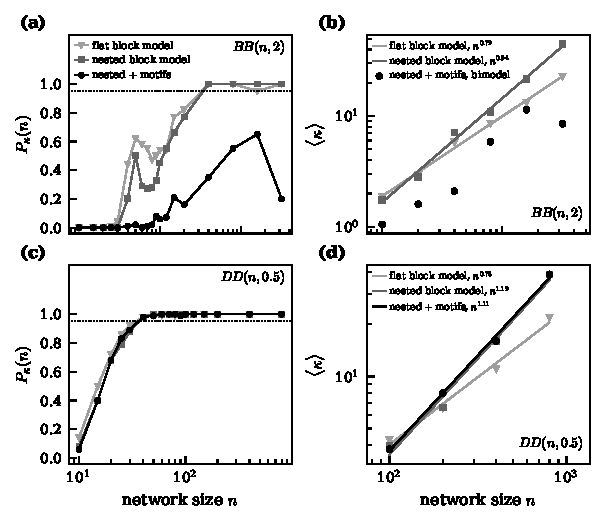
\includegraphics[width=\linewidth]{figs/fig-gr-squares.pdf}
  \caption{\textbf{Two rules built from squares, and only one of them says so.}
  Panels as in Figure~\ref{fig:gr-ramsey}: $P_\kappa$ from a hundred networks at
  each size up to $n=200$ and twenty above it. \textbf{(a)} $BB(n,2)$ closes one
  square per step on two new nodes, so its squares are nearly disjoint, the
  alphabet takes them up, and the communities the block model reports are largely
  dissolved. \textbf{(b)} $DD(n,q)$ at $q=\tfrac12$ closes squares in far
  greater numbers, but as overlapping $K_{2,d}$ bicliques rather than separable
  motifs; the alphabet plants none of them, and all three methods agree.}
  \label{fig:gr-squares}
\end{figure}

\section{The lattices that describe themselves}
\label{sec:gr-square}

Two lattices are left, and they are the ones on which the alphabet does the most
and the search does the worst. Taking them together is what empties the fractal
class and puts both of them in the first.

The pseudofractal web hangs a new node on both ends of every link, closing a
triangle; the diamond replaces every link by two parallel paths of one node each,
closing a square. Both reach exactly two steps --- every new node is adjacent to
nodes that were already adjacent --- and both rebuild the whole lattice at once,
which is what keeps their cycles clean, since a rule that subdivides one link at a
time stretches the cycles it has already made. They differ in the cycle they
close and in almost nothing else.

Fitted, they look like a clean contrast. Both sit at the modular limit under the
nested block model, $1.02$ and $1.05$, and under the motif alphabet the
pseudofractal reads $0.99$ while the diamond falls to $0.31$; the diamond's fit
returns $3$, $5$ and $7$ groups at $n=684$, $2732$ and $10\,924$, a count
climbing by a fixed amount while the lattice quadruples. That contrast was the
original reading of this section, and it does not survive.

\subsection*{Both lattices tile themselves exactly}

Each of these rules gives every existing link exactly one new motif per
generation. So the motifs closed at the \emph{last} generation have distinct old
links and disjoint new chains, and between them they use every link in the
network exactly once. A perfect edge-disjoint tiling of the lattice by its own
motif exists at every size, in both lattices, and it can be written down from the
construction without fitting anything: $729$ triangles for the $2187$ links of
the pseudofractal at $n=1095$, $1024$ squares for the $4096$ links of the diamond
at $n=2732$.

Price that decomposition and compare it with what the search finds:

\begin{center}
\footnotesize\setlength{\tabcolsep}{5pt}
\begin{tabular}{lrrrrrr}
\hline
 & & \multicolumn{2}{c}{as fitted} & \multicolumn{2}{c}{the tiling} & \\
lattice & $n$ & $\Sigma$ & $\kappa$ & $\Sigma$ & $\kappa$ & cheaper by\\
\hline
pseudofractal & $366$    & $4\,474$   & $5$  & $3\,887$   & $1$ & $587$\\
pseudofractal & $1\,095$  & $15\,428$  & $14$ & $13\,728$  & $1$ & $1\,700$\\
pseudofractal & $3\,282$  & $53\,082$  & $44$ & $47\,673$  & $1$ & $5\,409$\\
diamond       & $684$    & $7\,812$   & $3$  & $7\,434$   & $1$ & $378$\\
diamond       & $2\,732$  & $37\,213$  & $5$  & $35\,666$  & $1$ & $1\,547$\\
diamond       & $10\,924$ & $171\,368$ & $7$  & $166\,876$ & $1$ & $4\,493$\\
\hline
\end{tabular}
\end{center}

\noindent The tiling is cheaper at every size, on both lattices, by a margin that
grows with the network. Handed to the optimiser as a starting state it does not
move off it. And it uses \emph{one} community: a single block, every link spoken
for by a motif, nothing left for a partition to explain.

So on the criterion this chapter has used throughout, the best available
description of the pseudofractal web has no communities --- not the fourteen the
fit reports at $n=1095$, and not the forty-four it reports at $n=3282$ --- and the
same is true of the diamond. The two rules are in the same class. Their
description lengths are not merely similar but equal to the bit where their sizes
coincide, $7434$ at $n=684$ and $35\,666$ at $n=2732$, because both are tiled by
their own motif on the same $n$ and $m$.

\subsection*{What that costs, and what it does not}

It costs the contrast. The pseudofractal was this section's foil --- the lattice
that keeps its law while the diamond loses it --- and there is no such foil.
Along with it goes the argument that reach cannot be the discriminator because
two rules of equal reach end up in different classes: they do not end up in
different classes. Chapter~\ref{ch:communities}'s ranking of a triangle rule
against a square rule may still be telling us something, but not this.

It does not cost the finding. The diamond's own result is strengthened rather
than weakened: an alphabet can take a network's communities away entirely, and
under the best description available the diamond has none at all, rather than the
vanishing density earlier arithmetic gave it. What was reported as $\kappa$
growing like $\log n$ was a partition the search was carrying and did not need.

Nor does it touch the comparison that made the finding safe. Reducing the
alphabet to the link alone recovers the ordinary degree-corrected model exactly
(Section~\ref{sec:gr-motifsbm}), and on the diamond it costs $8908$, $41\,929$
and $198\,987$ bits at the three sizes against the motif description's $7434$,
$35\,666$ and $166\,876$ --- margins of a sixth rather than the eighth the fitted
comparison gave. The motif description wins by more than was claimed, not less.

The awkward part is what it says about the instrument. These are the two networks
in the book whose optimal description can be written down by hand, and they are
the two where the greedy search is furthest from it --- by up to a tenth of the
whole description length. That is not a coincidence, and
Chapter~\ref{ch:bubbles} takes it up: a deterministic rule builds an exact
optimum, and an exact optimum is a thing a greedy search can exactly miss. Every
other rule in this book is stochastic, lays its motifs across links chosen at
random, and has no such optimum to be missed.

\section{What decides the class}
\label{sec:gr-decides}

Three classes, and two rules that changed class when the vocabulary changed. What
is it about a rule that decides which way it goes?

Not the motif's shape: triangles dissolve nothing on local search or $BB(n,1)$
and everything on the pseudofractal, and squares dissolve everything on
$BB(n,2)$ and the diamond while doing nothing whatever on $DD(n,q)$ or
duplication--split. What the master table's last column measures is the one
quantity that separates the cases at the ends: how many of a network's links an
edge-disjoint decomposition can take up.

At one end sit the two lattices, at a hundred per cent. Each gives every link one
new motif per generation, so the last generation's motifs tile the whole network,
and a partition is left with nothing to explain --- which is exactly what the fit
finds when it is started from the tiling, one community and no residue
(Section~\ref{sec:gr-square}). At the other sits duplication--divergence at
nought per cent, where every square is stacked on the same shared neighbourhood
and a decomposition that gives each link to one motif can name almost none of
them; there the alphabet never engages and the partition keeps all of its work.

That is the mechanism where it can be seen cleanly. Where the motif tiles the
network, the partition has nothing left to describe and the communities go. Where
the motifs overlap, they cannot absorb what the partition was explaining, and the
communities survive. The same overlap that made duplication's bicliques
unnameable is here doing something useful.

Both ends are extremes, and it is worth saying what makes them legible. A
hundred per cent against nought is not a marginal gap, and the lattices are
deterministic --- one network per size, no sampling, and a decomposition that can
be checked by construction rather than searched for.

Between the ends the account has nothing to say, and the last column says so
plainly.
$BB(n,1)$ names $54\%$ of its links and keeps its communities; $BB(n,2)$ names
$57\%$ and loses them; local search names $62\%$, more than either, and is in no
danger at all. Three rules within eight points of each other on the quantity that
is supposed to be deciding, and two different outcomes. Whatever separates
$BB(n,1)$ from $BB(n,2)$, it is not how much of the network their motifs can take
up, and no reading of that column will supply it.

What does separate them is a question about the bubble family rather than about
this chapter's three classes, and the family repays being taken on its own terms:
$L$ is a dial, the rule is otherwise fixed, and the whole sequence can be fitted
with the alphabet extended to name each rule's own cycle. That is done
separately. What belongs here is the negative: the tiling account earns the two
lattices and does not earn the rest, and the difference between $BB(n,1)$ and
$BB(n,2)$ is left open by it.

What can be said from this side is what happens when nothing is taken up.
$BB(n,1)$ grows its communities as $n^{0.892}$ with the alphabet and $n^{0.886}$
without it, over $n=400$ to $3200$ --- indistinguishable. A motif the
decomposition cannot lay down over the network costs that network's density
nothing, whatever else is going on.

The caution generalises past any one rule. Wherever an alphabet can absorb the
same links that a partition would have explained, the two descriptions trade off
against each other, and the margin between them can fall below the
network-to-network scatter --- at which point the criterion still has a
preference but no single fit reliably reports it, and what comes back is decided
by where the search began. That is a limit on what any such method can be asked
to settle from one realisation, and not a defect of this implementation.
$BB(n,2)$ is that limit made visible: a real preference of a tenth of a bit per
node, carried on a scatter half again as large.

\begin{quote}
\emph{To follow up.} Chapter~\ref{ch:graphons} measured the community density of
three real growing networks with a vocabulary that could not name a triangle, and
the diamond shows that such a vocabulary can flatter a network into a density it
does not have. Whether the Internet and the yeast interactome keep $\beta=1$
under the full alphabet is being measured and is not settled here; the
collaboration graph, at sixty thousand nodes, is beyond what the motif fit can
reach at present. The interesting outcome would be the third class. A real
network landing at $\tfrac12<\beta<1$ and staying there under motif correction
would be the first genuinely fractal community structure in this book ---
Chapter~\ref{ch:communities}'s $0.61$ having turned out to be the flat model's
ceiling, and Chapter~\ref{ch:graphons}'s $0.80$ a sample that mixed grown
networks with catalogued ones.
\end{quote}

\section{Which change moves which number}
\label{sec:gr-doubledissoc}

Three methods have been compared through these sections, and they differ in two
ways rather than one. Flat against nested is a difference of resolving power and
nothing else; nested against nested-with-motifs is a difference of vocabulary and
nothing else (Section~\ref{sec:gr-motifsbm}). Reading the master table of
Section~\ref{sec:gr-classes} across rather than down, the two differences turn
out to move two different quantities, and it is worth separating them because
one of them is a great deal better behaved than the other.

Where the first difference comes from was the subject of
Chapter~\ref{ch:graphons}, and was priced there exactly: the two models express
the same partitions and differ only in what naming one costs, the flat model
paying a charge quadratic in the number of groups and so meeting
Eq.~\eqref{eq:gr-flatceiling}'s ceiling of $\sqrt n$, the nested model
compressing the group-level structure instead and reaching
Eq.~\eqref{eq:gr-nestedceiling}'s $n/\log n$. Nothing in that arithmetic mentions
what the links are made of.

\emph{Resolution moves the exponent, and only the exponent.} Going from the flat
model to the nested one lifts $\beta$ by two to four tenths on every rule in the
table without exception, and moves the onset $r_\kappa$ by at most a seventh ---
$70$ to $80$, $90$ to $100$, $400$ to $400$, $40$ to $40$. It never changes a
rule's class, because it cannot: the flat model's fractal-looking exponents are
its ceiling, and lifting the ceiling reveals the density that was there all
along.

\emph{Vocabulary moves the onset, and sometimes the class.} Naming a rule's own
motif moves $r_\kappa$ by a factor of two to four --- $80$ to $200$ for local
search, $100$ to $400$ for $BB(n,1)$, and at least four and perhaps sixteen for
the diamond, whose generations are too far apart to pin down --- and leaves it
untouched where the alphabet has nothing to name, as with duplication--split and
duplication--divergence. On the five random rules where the alphabet cannot take
up the whole network it leaves $\beta$ alone to within a hundredth or two. On the
three where it can, it does something the resolution
knob cannot do at all: it moves the rule out of the constant-density class
entirely --- $BB(n,2)$, the diamond and the pseudofractal all into the first,
with no communities left at all.

So the tidy statement --- one knob for how finely a network can be cut, another
for whether there is anything to cut --- holds for most of the table and fails in
exactly the cases this chapter was written about. The failure is not a
complication to be regretted; it is the finding. A vocabulary that
\emph{cannot} take up the whole network leaves the exponent alone, and that is
the common case. A vocabulary that can take up the whole network takes over the
description, and then the exponent is not measuring the network's communities any
more but the leftovers of a tiling.

The asymmetry has a reason. The exponent is a statement about how finely a
network can be cut, and nothing about the vocabulary for describing links changes
how many groups a method is \emph{able} to resolve --- that ceiling is fixed by
what the description length charges for the block structure. But the vocabulary
does change how many groups are \emph{worth} resolving, by offering an
alternative account of the same links; and where that alternative can cover
everything, the number of groups worth resolving falls to almost none. The
ceiling and the demand are different things, and only the second is open to the
alphabet.

This also tidies up a conclusion that has been uncomfortable since
Chapter~\ref{ch:graphons} drew it: that Chapter~\ref{ch:communities}'s exponent
is in part a statement about the flat block model rather than about the networks.
It can now be said without reference to motifs at all. On the rules where the alphabet cannot tile, it is
irrelevant to $\beta$; the whole of the shift from $0.61$ is the nested model,
which is a standard tool and not one invented here. Whatever else is uncertain
about the machinery of these sections, that conclusion does not rest on it.

And it answers, with one qualification, the question Chapter~\ref{ch:graphons}
left at its door. What that chapter found was a density: with the resolution
lifted, the number of communities grows in proportion to the size, so $b=B/n$
becomes a number a network has rather than a rate at which something grows. The
obvious worry about such a quantity is that it might be an artefact of a poor
vocabulary --- that a model forced to describe every triangle as three separate
links would invent communities to absorb what it could not name, and that a
richer alphabet would dissolve them. On the rules whose motifs overlap it does
not: give the model triangles, squares and bicliques and the density stays where
the nested prior put it. The qualification is the three rules whose motifs do not
overlap --- $BB(n,2)$ and the two lattices --- where exactly that worry is
realised, and it is why Chapter~\ref{ch:graphons}'s conjecture has to be read as
a claim about the best available description rather than about the network
itself.

Two instrument effects had already been found and separated before this chapter
began, and it is worth noticing that all three were found the same way.
Chapter~\ref{ch:communities}'s $0.61$ became $0.80$ when the prior stopped
charging quadratically for groups, and $0.80$ became $1$ when the sample stopped
mixing grown networks with catalogued ones. Neither move was about networks. What
this chapter adds is a third of the same kind and a sharper one: change the
vocabulary and a network can change not merely its exponent but the class it
belongs to. A limit class, like an exponent, is a property of a network together
with the code used to describe it.
